\par{Another poor performance metric was the L1 hit ratio, indicating the 
    fraction of successful L1 cache accesses. Ideally, the L1 hit ratio 
    should be as close to 1 as possible. In some cases, a high L1 hit 
    ratio is achieved, but in other cases, a very low L1 hit 
    ratio appears. This indicates that the algorithm is not always 
    using L1 cache effectively. For example, with a block size of 32, 
    the perimeter \emph{kernel} achieved an L1 hit ratio of 0.646 and the 
    internal \emph{kernel} had an L1 hit ratio of 0.490, which is well 
    below what can be achieved and highlights an inefficiency in 
    the algorithm. Also, for the same block size, the estimated latency 
    impact was very high. The estimated latency impact is a metric that 
    gives the average number of cycles that are taken to service L1 
    cache misses. The estimated latency impact was 423.337 for block 
    size 32. So, not only are the attempts to access data missing L1 
    cache for large portions of the time, but it is likely that they 
    are also missing L2 cache.}

\par{From analysing the assembly code some important results appear. 
    There are a few key instructions to note. In this section of 
    assembly code, there are two prefetching instructions.}

\begin{itemize}
    \item \textbf{\emph{vprefetch0}:} prefetching from global memory to L1 cache.
    \item \textbf{\emph{vprefetch1}:} prefetching from global memory to L2 cache.
    \item \textbf{\emph{vloadunpackld/vloadunpackhd}:} pack vector registers 
        with data from cache.
\end{itemize}

\par{Figure \ref{Assembly_64} shows the assembly code from the internal 
    kernel with block size 64. There are prefetching instructions 
    for both L1 and L2 caches, which is expected since the data required 
    for all the \emph{work items} in a \emph{work group} should exceed the size of 
    L1 cache. Some data should be stored in L2 cache. Unsurprisingly, 
    the prefetching instructions account for the 
    bulk of the computation time.}

\begin{figure}[!h]
    \centering
    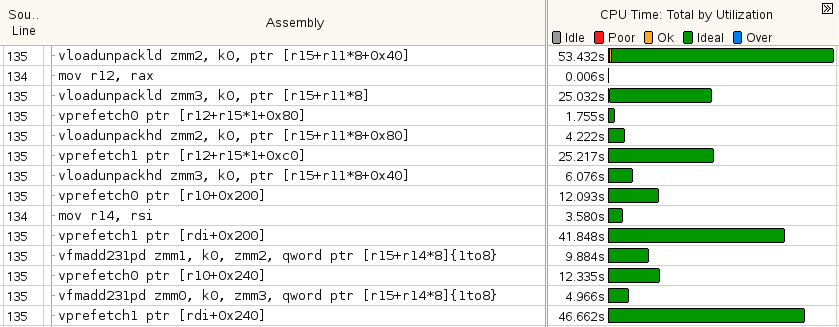
\includegraphics[width=0.6\textwidth]{figures/Assembly_64.png}
    \caption{Assembly code for internal \emph{kernel}, block size = 64.}
    \label{Assembly_64}
\end{figure}

\par{Figure \ref{Assembly_2} shows the assembly code for the internal \emph{kernel} with 
    block size of 2. In this case, all the data required by the \emph{work items} in 
    the \emph{work group} should easily fit in L1 cache. However, the prefetch1 
    command is still being used. Thus, even with small data sizes, L2 cache 
    is being used to store the data. Clearly, there is some problem with 
    the memory management.}

\par{In the case of block size 2, there is also far more prefetching 
    instructions, which highlights the possible overhead of choosing 
    a small data size for each \emph{work group}.}

\begin{figure}[!h]
    \centering
    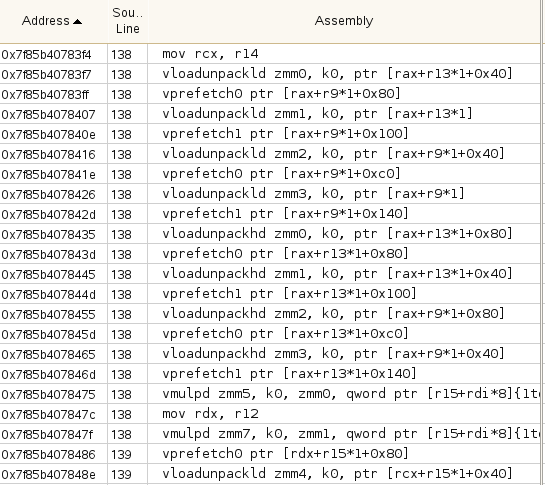
\includegraphics[width=0.6\textwidth]{figures/Assembly_2.png}
    \caption{Assembly code for internal \emph{kernel}, block size = 2.}
    \label{Assembly_2}
\end{figure}


